\section{\heiti{问题背景阐述}}

论文的第一部分是问题背景阐述。主要说明研究问题的背景来源、目前的主流解决策略、本项目采用的解决方式
以及后续可能出现的前景和困难等。这一部分本论文将详细解释 FIR 滤波器的原理、离散傅立叶变换的原理和计算机
实现、信号处理算法中的乘法器性能等内容。最后我们将简要说明本项目如何分别解决此次比赛中题目的三个技术诉求。

\subsection{\heiti{有限脉脉冲响应滤波器(Finite Impulse Response Filter, FIR Filter)}}
工程上进行 FIR 滤波器(FIR Filter,以下简称FIR或FIR滤波器)是非递归型滤波器的简称,全称是有限长单位脉冲响应滤波器
(Finite Response Filter)。

滤波器是对波动信号进行处理的基础器件,工程上需要对信号(诸如电磁波、声波、辐射光谱等随时间波动变化信号)进行
采样,得到随时间变换的采样信号序列。数学上抽象成一族点或自然数集上的函数 $\left\{z_{nT}\right\}_{n\in\N}$。
这里 $T$ 是采样周期,在一个采样周期中通常认为波形在基频 $\omega$
的倍频上的能量分布是不随时间变化的,不同采样周期的频谱能量分布可能有变化。

数学上看 FIR 滤波器是一些重要信号处理变换(诸如 Laplace 变换/ Fourier 变换等)的近似情况下推广,其数学核心是
如下的 $Z$-变换。
\paragraph{\heiti{Z-变换(Z-Transformation) 和卷积(Convolution)}}
有限长单位脉冲响应滤波器(以下简记为 FIR 滤波器)数学上通常抽象成是一系列(有限长度) $Z$-变换如下
\begin{align*}
    &H(z) = \sum_{n=0}^{n=N} h(n) z^{-n},\quad z \in \mathbb{C}\\
    &(\text{或} H(z) = \sum_{n=N_1}^{n=N_2} h(n) z^{-n},\qquad N_1, N_2 \in \N),\qquad \tag{A1}
\end{align*}
其中 $h(0),..,h(n)$ 是滤波器的脉冲响应序列(Impulse Response Sequence)。
在 FIR 滤波器的设定中这是一个有限的序列(一般而言从零到一个正整数 $n$,称为
 FIR 滤波器的阶数),从而 FIR 中的有限长单位因此得名。
而乘数 $z \in \C$ 是一个标准的复数,用来表示处理信号采样的频率信息。 $z$ 通常可以随时间变化但是在
一般是采样周期内假设是基频 $\omega$ 的常系数幂级数(含时 Fourier 分析或构建语谱图(Spectrogram)的工程要求),
即 $z_{nT} = \sum_{k\in\Z} a_{n,k} e^{-\sqrt{-1}k \omega },\quad \forall t\in \R^+, n\in \N^+$

特别地如果 $z = e^{\sqrt{-1}\omega}$ 是 Dirac 脉冲函数的 离散 Fourier 变换 (DFT),即一些特殊波形的频谱时
无截断的 $Z$-变换时,有
\begin{eqnarray*}
    &H(z) := \sum_{n > -\infty}^{n <+\infty} h(n) z^{-n}\\
    &\Rightarrow H(e^{\sqrt{-1}\omega}) =\sum_{n > -\infty}^{n <+\infty} h(n) e^{-\sqrt{-1}n \omega}
    = \widehat{h} (\omega)
\end{eqnarray*}
恰好是无截断的 DFT。(对 $h$ 进行有限长度截断从而得到有限长度的 DFT)

进一步考虑 $(A1)$。如果考虑一段频率信号 $X(z) = \sum_{n\in\Z} x(n) z^{-n}$,那么其在一个
$(A1)$ 形式的 FIR 滤波器作用下得到频率响应 $Y(z)$ (或者等价地称为脉冲响应,Impulse Response/Frequency Response)应该是
\begin{eqnarray*}
    Y(z) = H(z)X(z),\qquad z = e^{-\sqrt{-1}\omega}(\text{或其他形式的频谱})\\
    Y(z) = \sum_{n\in \Z} y(n)z^{-n},\qquad y(n) = \sum_{k=0}^{k=N}h(k)x(n-k),\quad \forall n\in \Z
\end{eqnarray*}
于是计算滤波器输出的频率响应 $Y(z)$ 的各分量(各倍频的能量分配)是
\begin{equation*}
    y(n) = \sum_{k=0}^{k=N}h(k)x(n-k),\quad \forall n\in \Z,\qquad \tag*{(A2)}
\end{equation*}
因为这代表了滤波器的理论输出,从而通过式 $(A2)$ 可以计算每一个倍频上分配的多少能量。抽象到数学上
这是给定输入序列 $\left\{x(n)\right\}_{n\in\Z}$ 和有限卷积序列 $\left\{ h(k)\right\}_{k\in \left\{0,..,N\right\}}$
进行卷积运算(Convolution Operation)。

从上述的数学表示可知,一个 FIR 滤波器的硬件算法性能,最底层运算速度上是受以下两方面制约

\begin{itemize}
    \item \heiti{第一个公式 $(A1)$ 中的 $z^{-1}$-乘法器的性能}。这部分对应 FIR 滤波器的真实输出。
    \item \heiti{第二个公式 $(A2)$ 中的卷积操作的性能}。这部分对应滤波器的理论输出。
\end{itemize}

通常而言卷积运算中涉及分量错位乘法时也会加入硬件实现的高精度-高精度乘法的性能,由于 $(A1),(A2)$
完全表示相同的频谱信息,本项目主要大力优化卷积操作的性能来实现华为``低功耗自适应 FIR 滤波器''难题的技术诉求。

除此之外,滤波器本身在硬件上的实现要适应硬件自身的条件,例如不同硬件的基础运算性能不尽相同、不同硬件的内存管理资源调度
的性能也不尽相同。以下简要通过 \href{https://schaumont.dyn.wpi.edu/ece4703b20draft/lecture4.html}{网络资料}
简单解释这两点。

\paragraph{\heiti{滤波器的架构优化}}
FIR 滤波器大概有如下四种不同的架构实现。本项目通过综合如下四种架构的优劣开发出自行的架构。这将在论文的第三部分说明。

第一种是直接形式(Direct-form)。其带有常数系数的滤波器数据流程图如下图\ref{fig:Direct-form-FIR}所示。
\begin{center}
    \begin{figure}[ht!]
        \begin{subfigure}{\textwidth}
            \centering
            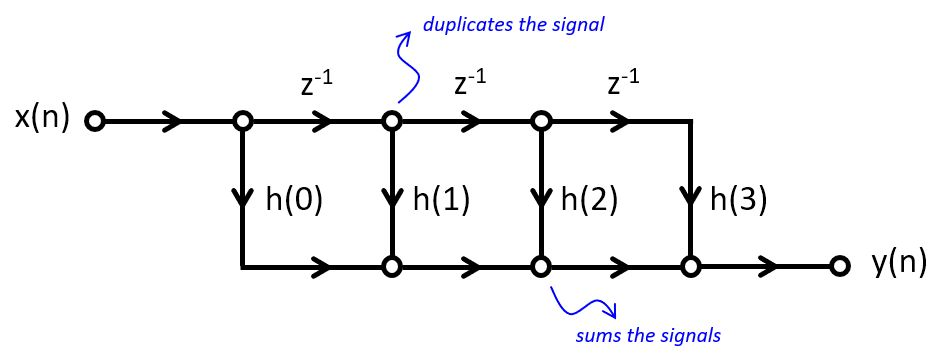
\includegraphics[scale=0.3]{figures/FIR_Direct.jpg}
            \caption{直接形式 FIR 滤波器 (阶数 $n=4$)}
            \label{fig:Direct-form-FIR}
        \end{subfigure}
        \hfill
        \begin{subfigure}{\textwidth}
            \centering
            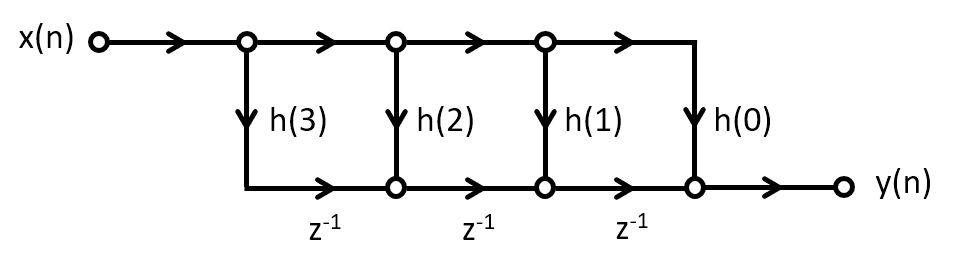
\includegraphics[scale=0.3]{figures/FIR_Transpose.jpg}
            \caption{反向形式 FIR 滤波器 (阶数 $n=4$)}
            \label{fig:Transpose-form-FIR}
        \end{subfigure}
        \caption{两种基本 FIR 架构}
        \label{fig:Direct-Transpose-FIR}
    \end{figure}
\end{center}

从图中可以看出直接形式滤波没有对架构作任何优化,将会进行 $n+1$ 次常系数 $z^{-1}$-乘法和 $n$ 次加法。
其中 $n$ 是滤波器阶数,那么进行完整的 FIR 滤波信号处理的时间复杂度至少是 $\O (n^2)$ (假设乘法复杂度和加法相同)。

和直接形式相反是反向形式(Transpose-form)即上述\ref{fig:Transpose-form-FIR}。注意此时的乘法器的系数正好和直接形式实现相反。相比于直接形式
反向形式没有复生信号的操作,而是并行处理信号后累加。于是对于并行计算性能好的硬件,反向形式架构的滤波器性能更好。

而事实上硬件上高精度乘法要比加法慢很多,如果能够在架构设计上减少乘法次数将有效地提升滤波器性能。后续的层级形式
(Cascade-form)和频采形式(Frequency Sampling)均是基于这种思想。首先考虑层级形式,考虑 $Z$-变换的 Laurent 
多项式以 $z^{-1}$ 变量因式分解得到
\begin{equation*}
    H(z) = \sum_{n=0}^{n=N}h(n)z^{-n} = h(0)\prod_{k=1}^{k=N}(1- a_k z^{-1}) = \prod_{k=1}^{k=N} G_k (z)
\end{equation*}
这里 $a_k \in \C, k=1,..,N$ 是一些和 $H(z^{-1})$ 的零点的倒数。那么安装滤波原理可以逐次实现
$G_1(z),..,G_k (z)$ 的滤波器再将它们串行处理。特别地如果 $\left\{h(n)\right\}_{n\in\N}$ 是实数序列
那么根据复根成对原理可以将 $H$ 分解为一些至多二次因子的乘积。从而在串行处理的滤波器中只包含实数乘法。这样作降低
了复数乘法的次数,提高了性能。下图是一个按上面论证实现的 FIR Cascade-form Filter。
\begin{center}
    \begin{figure}[ht!]
        \centering
        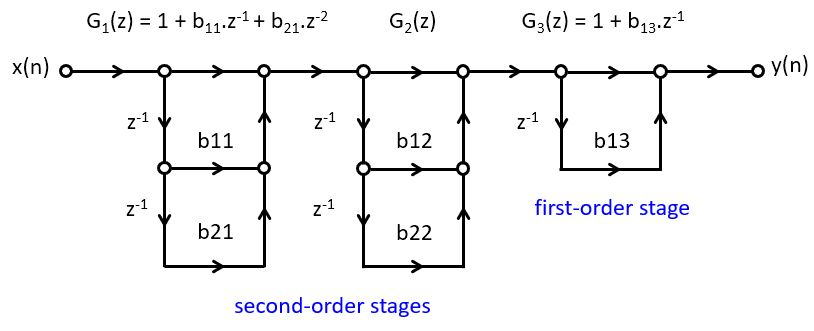
\includegraphics[scale = 0.5]{figures/FIR_Cascade.jpg}
        \caption{层级形式 FIR 滤波器 (实数化乘法)}
        \label{fig:Cascade-form-FIR}
    \end{figure}
\end{center}
层级形式将阶数较高的 FIR 滤波器分解成小阶数的子滤波器,此设计可以模块化架构从而增大数据吞吐量。可以说有一定功能。
最后一种架构是功能性架构即频采架构(Frequency Sampling)。其来自于物理学中的共振器/共鸣器(Resonator),作用是在
特定频率上放大其幅度/振幅。$Z$-变换结构是
\begin{equation*}
    H(z) = \frac{z^2}{z^2 - 2 \cos \theta z + 1} = \frac{1}{1 - 2\cos \theta z^{-1} + z^{-2}} = \frac{1}{X(z)} \qquad \tag{A3}
\end{equation*}
这里 $\theta$ 通常和共振频率 $\omega$ 相关,而其反方向是实现是一种频率梳(Comb)。滤波器结构是形如
\begin{equation*}
    H(z) = 1 - z^{-m},\qquad \tag{A4}
\end{equation*}
$(A4)$ 的 $Z$-变换通常会将频率为 $m$ 间隔的局部响应消除从而呈现如下的梳状结构(\ref{fig:FIR-Comb})。事实上 $(A3)$ 的 $H(z)$ 可以
写成频率梳的某种逆变换(按式 $(A3)$)。
\begin{center}
    \begin{figure}[ht!]
        \begin{subfigure}{\textwidth}
            \centering
            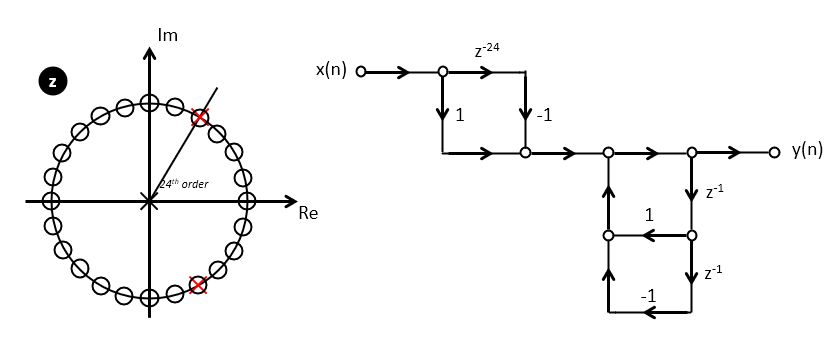
\includegraphics[scale=0.4]{figures/FIR_Frequency.jpg}
            \caption{频率采集 $H(z) = 1-z^{-24}$}
            \label{fig:FIR-Frequency}
        \end{subfigure}
        \hfill
        \begin{subfigure}{\textwidth}
            \centering
            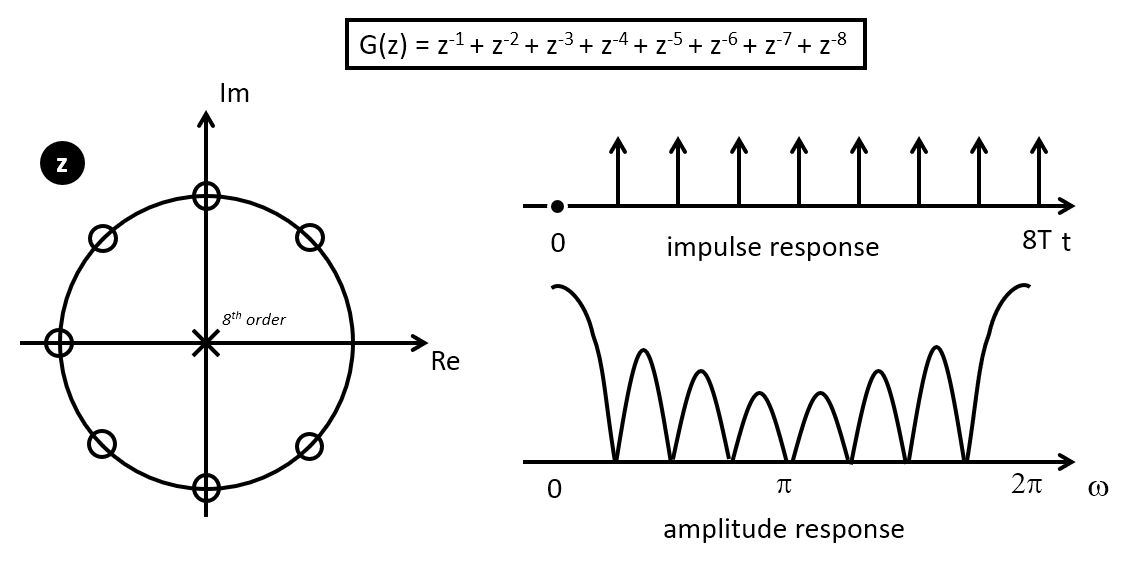
\includegraphics[scale=0.4]{figures/FIR_Comb.jpg}
            \caption{频率梳的效果}
            \label{fig:FIR-Comb}
        \end{subfigure}
    \end{figure}
\end{center}
另外,如果响应序列 $\left\{h(n)\right\}_{n}$ 具有一定的对称性,通过更聪明的办法可以设计乘法器更少的架构以提升性能。
例如 \ref{fig:FIR-Optimizing} 中 $h(n-k) = h(k),\forall k\le n$ 是中心对称的,那么通常的直接实现可以改成系数乘法次数减半的对称架构如
\begin{center}
    \begin{figure}[ht!]
        \centering
        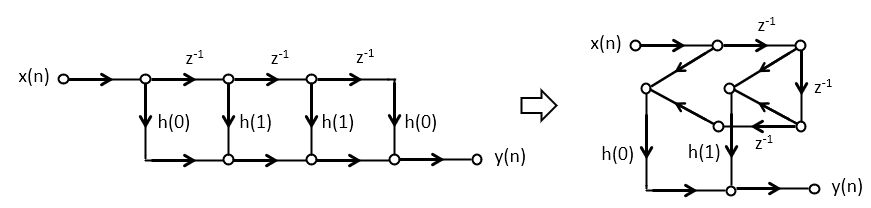
\includegraphics[scale=0.6]{figures/FIR_Optimizing.jpg}
        \caption{减少系数乘法个数}
        \label{fig:FIR-Optimizing}
    \end{figure}
\end{center}
另外如果 $h(n)$ 中有公共间距数字例如 $3 = 1+2 , 5 = 1+ 2+ 2$ 时可以通过只计算 $\times 2$乘法然后累加的方式降低
乘法器算力负担。

\paragraph{\heiti{滤波器中的内存管理}}

经过上百次系数乘法计算后 FIR 设计可能变得相对复杂很多。因此在某种意义上对 FIR 滤波器硬件进行内存管理尤为重要。
详细的字典级资料此处建议参考\cite{Parhi2007}。本处只指出关于缓存管理的本项目优化方式。
即将信号延迟处理的缓存移位操作优化成指标计算的旋转操作。
示意图如\ref{fig:Buffer}。
\begin{figure}[ht!]
    \centering
    \begin{subfigure}{0.35\textwidth}
        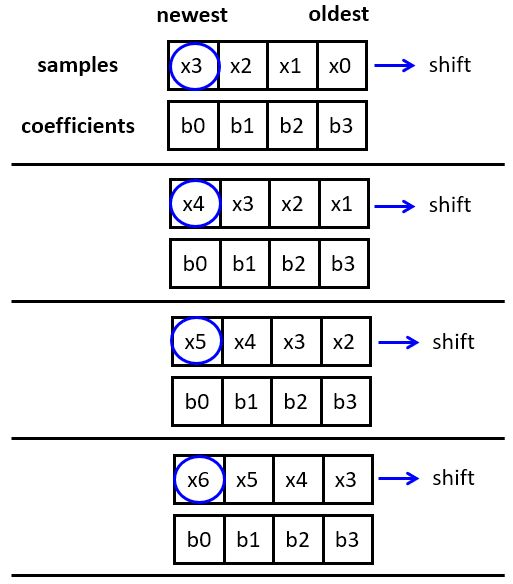
\includegraphics[width=\textwidth]{figures/Shift.jpg}
        \caption{缓存Shift操作}
        \label{fig:Shift}
    \end{subfigure}
    \hfill
    \begin{subfigure}{0.35\textwidth}
        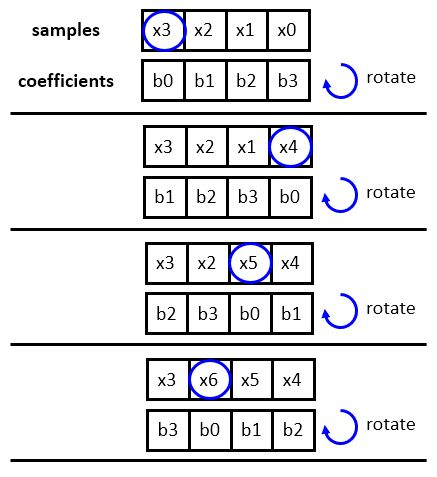
\includegraphics[width=\textwidth]{figures/Rotation.jpg}
        \caption{缓存旋转操作}
        \label{fig:Rotation}
    \end{subfigure}
    \hfill
    \caption{内存管理优化}
    \label{fig:Buffer}
\end{figure}

其效果参考如下表格。
\begin{table}[ht!]
    \begin{center}
      \caption{性能比较}
      \label{tab:Buffer-Comparison}
      \begin{tabular}{l|c|c|c} % <-- Alignments: 1st column left, 2nd middle and 3rd right, with vertical lines in between
        \textbf{FIR Design}     &\textbf{16 taps}   &\textbf{32 taps}   &\textbf{64 taps}\\
        \hline
        tap-shift               &383                &703                &1343\\
        circular buffer         &306                &530                &913\\
        throughput (circular)   &1.25x	            &1.32x              &1.47x\\
      \end{tabular}
    \end{center}
\end{table}

最后对于更加详细的信号处理介绍,尤其是滤波器的简要介绍本文采用了\href{https://schaumont.dyn.wpi.edu/ece4703b20draft/index.html#}{此课程页面}为主要
参考资料。其为伍斯特理工学院的``实时信号处理 B'' (Real Time Digital
Signal Processing B Term)课程。

\subsection{\heiti{离散傅立叶变换及快速实现(Discrete/Fast Fourier Transformation, DFT/FFT)}}

在上一节中 $(A2)$ 涉及到卷积算法的快速实现。实际上考虑最简单情形的两个同次数多项式乘法
\begin{align*}
    &A(x) := \sum_{n=0}^{n=N}a(n)x^n,\qquad B(x) := \sum_{n=0}^{n=N}b(n) x^n,\qquad N \in \N^+\\
    &C(x) := A(x)B(x) = \sum_{n=0}^{n=2N} c(n)x^n
\end{align*}

乘法结果中 $C(x)$ 的各项系数 $c(n)$ 不难计算出是 $\left\{a(n)\right\}_{n=0,..,N}$ 和 $\left\{b(n)\right\}_{n=0,..,N}$
的卷积和(或卷积的某处值)形如
\begin{eqnarray*}
    c(n) = \sum_{k=0}^{k=N}a(k)b(n-k),\qquad n=0,..,2N
\end{eqnarray*}
由于多项式可以被其各项系数唯一决定,离散卷积算法等价于多项式乘法系数计算算法,也就是说求序列的离散卷积和求两个多项式乘积的
系数一样困难(在算法理论上看这两个问题是等价的)。

根据上面计算如果用多项式系数存储多项式,计算多项式乘法的复杂度大概是 $\O (n^2)$ (因为计算 $n$ 个乘积系数,每一个系数平均要进行 $\frac{1}{2}n$ 次乘法和加法)。
那么这是可以在时间复杂度上优化的吗?考虑著名的 Lagrange 插值公式,一个 $n$ 次多项式在 $n+1$ 个点的取值唯一确定了这个多项式。
具体表达式是 
\begin{equation*}
    F(x) = \sum_{k=0}^{k=n} F_k \prod_{i=0,i\not=k}^{i=N}\frac{(x- x_i)}{(x_k - x_i)},\qquad \mathrm{where}\, F(x_k) = F_k,\, k=0,..,N
\end{equation*}
如果考虑 $\left(F(x_0),...,F(x_n)\right)$ 表示多项式 $F$ 则另一个多项式 $G \sim \left(G(x_0),..,G(x_n)\right)$
同样表示。此时计算 $F,G$ 乘积只需要 $n$ 次乘法即
\begin{equation*}
    FG \sim \left(F(x_0)G(x_0),...,F(x_n)G(x_n)\right)
\end{equation*}
如果能以时间复杂度小于 $\O(n^2)$ 的算法从多项式系数计算出其在选定的 $n+1$ 个点的数值及此过程的逆运算,那么定点表示的多项式乘法
算法就在性能上(至少运算速度)超过普通乘法。
记 $N = \deg F$。从离散傅立叶分析的观点如果取 $x_k = e^{-\frac{2\pi \sqrt{-1}}{N+1}k}$,那么可知
\begin{equation*}
    F(x_k) = \sum_{n=0}^{n=N} f(n)x_k^n = \sum_{n=0}^{n=N}f(n)e^{-\frac{2\pi\sqrt{-1}}{N+1} kn}, k=0,..,N
\end{equation*}
于是 $F(x_k) = \widehat{f}(k)$。即在上述选定点下,多项式的定点序列是系数序列的离散傅立叶变换(DFT)。
那么系数序列此时是定点序列的离散傅立叶逆变换(Discrete Inverse Fourier Transformation,DIFT)。
于是如何快速计算 DFT 称为快速卷积、多项式快乘甚至随机变量分布计算或数论算法等领域的核心问题。
而第一个快速实现 DFT 的算法是基于分治思想的 Cooley-Tukey Scheme。

Cooley 和 Tukey 是 Princeton大学的两位数学家和计算机科学家,他们在二十世纪利用快速实现的离散傅立叶变换算法(Discrete Fourier Transformation/ Fast Fourier Transformation, Discrete
 Fourier Transformation with Fast ImplementationDFT/FFT)。时间复杂度可以达到 $\O (n \ln n )$。
此方式适用于 $n= 2^m$ 时,本项目实现方式主要参考了算法导论一书的 FFT 章节见
 \cite[Polynomials and FFT]{Cormen2022} 和 \href{https://en.wikipedia.org/wiki/Fast_Fourier_transform}{Wikipedia}。

对于 $n \not= 2^m$ 的多项式乘法或卷积,总可以通过引入先导零/占位的方式约化到 $n = 2^m$ 的情形,由于 $k$ 和 $2k$ 中必然有
一个 $2$ 的次幂,理论上快速傅立叶变换的时间复杂度不会超过 $\O (2n \ln n)$。另外 Cooley-Tukey 的变形中会处理 $N_1 N_2$ 阶数 FFT,
通常分解为 $N_1$ 个 $N_2$ 阶 FFT处理($N_1 \ll N_2$)。参看本文第二、第三部分。

\subsection{\heiti{信号处理算法中运算器性能}}
实时信号处理中提取的时间/频率信号(如 $u_t$ 或者 $z_t$)通常而言取值在一个高精度的浮点数集合上,例如
C/C++ 中的 float\_32 或 float\_64 等不同位数的浮点数。工程原理上来说,计算机(``朴素''的计算机,不包括例如 Wolfgang Mathematica 此种
存储实现任意精度的实数计算算法和诸多几乎``完全精度''的计算数学全套算法的超级计算机代数系统)无法实现
任意精度的数值计算,因为内存的有限性和很多计算过程实现时的限制。事实上 $64$ 位的高精度浮点数在信号处理上已经
非常够用了,而且为了集成到硬件,综合考虑性能、稳定性等因素,滤波器中的乘法器构件的实现,往往还需要舍弃一定精度
作近似计算。另外,一些更复杂的运算器例如卷积、内积、张量乘等运算,其优先级一般低于
常数乘法或浮点数乘法,但是不同实现方式的性能不尽相同。通常用执行一次运算器使用的基础乘法次数和基础加法次数
带上权重(表示单次乘法的平均耗时或资源开销)来衡量运算器的性能。如
\begin{eqnarray*}
    P_{\mathrm{op}} := N_{\mathrm{mul}} w_{\mathrm{mul}} + N_{\mathrm{add}} w_{\mathrm{add}} + P_{\mathrm{sche}}
\end{eqnarray*}
上面的 $P_{\mathrm{sche}}$ 是硬件的调度性能指标,本项目尽可能将这个指标拟合为和缓存量、I/O吞吐量相关的近真实指标。
不仅是硬件、算法层面上度量运算器的性能也尤为重要。在本论文的第四和第五部分,我们团队采用了上述指标对算法进行了测试
,并记录描述了结果。

\subsection{\heiti{技术诉求}}
针对华为领航杯应用数学大赛的难题七``低功耗自适应 FIR 滤波器''有如下三个主要技术诉求。
\begin{enumerate}
    \item \heiti{诉求一}:通过改变滤波器架构设计等办法,使得其硬件算法整体性能提升40\%。
    \item \heiti{诉求二}:指定位宽下引入近似乘法,实现乘法资源降低50\%,误差或信噪比(SNR)大于 $75 \mathrm{dBc}$
            ;或者使用机器学习模型训练,使得其训练
            性能基本无损($< 0.1 \mathrm{dB}$)
    \item \heiti{诉求三}:``低位宽'' FIR 滤波器算法实现($< 6 \mathrm{bit}$),并能够实现模型稳定校正且性能基本无损($< 0.1 \mathrm{dB}$)
\end{enumerate}

\paragraph{\heiti{诉求一}}
就本团队理解衡量 FIR 滤波器的整体性能指标可以使用功耗面积度量。

\paragraph{\heiti{诉求二}}
本项目通过基准测试方案在仿真机上对 FIR 滤波算法进行测试。主要指标为(参考刘伟强等人综述\cite{Liu2019})信噪比
\begin{equation*}
    \mathrm{SNR} := 10 \log_{10} \left[\frac{\max_{i}|\mathrm{AR(i)}|^{2}}{\frac{1}{N}\sum_{i=0}^{N-1}
    |\mathrm{AR(i) - ER(i)}|^{2}}\right]\qquad \tag{A5}
\end{equation*}
其中 $\mathrm{RR(i)}$ 是真实(近似)结果,$\mathrm{ER(i)}$ 是全精度结果。后续部分将着重测试此指标。

\paragraph{\heiti{诉求三}}
通过理论计算确定实现位宽的理论值应该为 $12 \mathrm{bit}$。
通过更大量的 ``代价权衡'' 将滤波器的位宽降低到 $6 \mathrm{bit}$,本项目后续将采用自适应机器学习预测的办法完成此诉求。

在本文第二部分经典方法复现中,三个子节将会依次详细论述本项目对上述三个诉求的经典解决方式。

在第三部分``理论和算法''中本文将尽可能清晰地叙述项目中使用的关键算法理论,具体创新和优化的细节部分。

在第四部分``实验数据及软硬件介绍''和第五部分``实验结果及主要结论''中本文将展示根据前三部分的算法理论实现的工程在仿真环境
的测试数据以及指标比较。

最后关于项目的复现以及移植,完整的源代码解释和运行环境信息全面呈现在附录一节。

